43. $\cfrac{1}{x+2}+\cfrac{1}{x+3}\geqslant\cfrac{1}{x}\Leftrightarrow \cfrac{x(x+3)+x(x+2)-(x+3)(x+2)}{x(x+2)(x+3)}\geqslant0\Leftrightarrow$\\$
\cfrac{x^2+3x+x^2+2x-x^2-2x-3x-6}{x(x+2)(x+3)}\geqslant0\Leftrightarrow\cfrac{(x-\sqrt{6})(x+\sqrt{6})}{x(x+2)(x+3)}\geqslant0.$\\ Применив метод интервалов, найдём ответ:
\begin{figure}[ht!]
\center{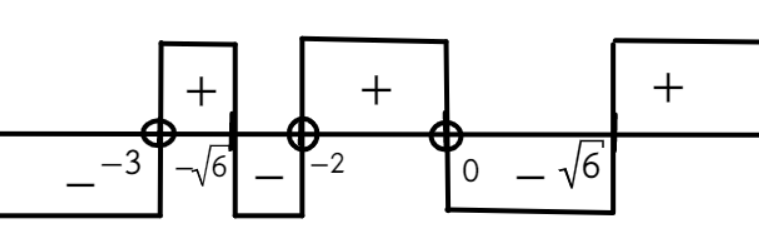
\includegraphics[scale=0.35]{int43.png}}
\end{figure}
$x\in(-3;-\sqrt{6}]\cup(-2;0)\cup[\sqrt{6};+\infty).$\\
